\documentclass[../main.tex]{subfiles}

\begin{document}
	L'application Android, nommée Equity, a été développée sous l'IDE Android Studio 3, avec l'API Android 16, supportant ainsi près de 99\% des appareils Android en circulation. Le code de l'application a été entièrement géré avec Git et est d'ailleurs disponible à l'adresse suivante : \url{https://github.com/tndnc/pandroid/tree/master/equity}. 
	
	L'application devait répondre aux spécifications suivantes: permettre aux utilisateurs de sélectionner des niveaux, de les résoudre et d'en noter la difficulté. Pour les administrateurs il était également important de pouvoir facilement mettre à jour la liste des niveaux ainsi que de pouvoir récupérer les notes et meta-données issues de son utilisation par les utilisateurs. Ces données devaient pouvoir être exportées vers une base de données.
	% Google sheets API v4 à ajouter dans partie sur google sheet.
	
	\subsection{Conception de l'interface}
	
L'interface centrale de l'application, l'aire de jeu d'Equity, est un des composants principaux du projet et a donc suivit un certain nombre d'itérations qui seront décrites dans la partie suivante. Le premier objectif de cette interface était de pouvoir représenter le jeu sur un écran de smartphone en mode portrait. En outre, il était important de réfléchir aux différents menus de l'application et au tutoriel permettant d'expliquer le jeu.

Ayant suivi en parallèle l'UE d'IHM pendant ce semestre, nous avons pu acquérir les connaissances et pratiques appropriées pour la conception de notre interface. Ces connaissance nouvellement acquises ont été appliquées tout au long du processus.

Il fallait tout d'abord identifier l'utilisateur qui était visé par notre application, mais nous nous sommes très rapidement rendu compte que cette notion était intrinsèque au sujet de notre projet. En effet, rappelons nous qu'il fallait évaluer la difficulté de nos niveaux et comparer nos prédictions à de vraies données. Or la notion de difficulté est subjective à n'importe quel être humain. Il nous fallait donc des données comprenant un maximum de diversité c'est-à-dire des utilisateurs de tous âges, de toutes formations, etc. L'idée était de minimiser le biais de nos résultats. Nous nous sommes donc donnés pour but de créer une application pour tout type d'utilisateur et l'interface devait aller dans ce sens aussi. Notre premier objectif était d'établir les besoins utilisateurs et tâches de notre système.

	\subsubsection{Les besoins utilisateur}

Afin de définir les besoins, il est de convention d'interviewer des utilisateurs potentiels pour comprendre leur réaction face au jeu. Un petit nombre de personne ont été consultées et confrontée au problème, initialement sous la forme visualisée en~\Cref{sec-analyse} (c'est-à-dire un graphe liant les agents avec des listes de préférences triées de haut en bas). Puisqu'aucune problème de compréhension n'était apparent à ce stade, les premiers prototypes de l'interface se sont donc vu largement inspirés par cette visualisation. Nous avons aussi étudié les interfaces de jeux mobiles populaires telle que Candy Crush ou encore 2048 pour mieux comprendre les caractéristiques d'une bonne interface. Ces données une fois regroupées nous ont permis de dégager plusieurs lignes directrices pour notre interface.

Lors de nos interviews nous avons demandé quelles étaient les caractéristiques d'un bon jeu d'après nos utilisateurs potentiels et l'un des points positifs le plus souvent pointé du doigt était la facilité avec laquelle un utilisateur comprenait les règles. Beaucoup se sont en effet plaint de la difficulté à \textquote{entrer} dans un jeu dès lors que la prise en main devenait difficile et que les règles étaient complexes. Or la notion de jalousie évoquée précédemment n'est pas forcément naturelle, il était donc crucial pour notre application d'avoir une interface la plus claire possible pour la compréhension du jeu. Toujours en rapport avec le premier souci, nous avons également remarqué au cours de nos recherches, que la quantité d'information à l'écran était un facteur important. Il apparaît que le sentiment de confusion est amplifié lorsqu'un nombre important de données s'affiche en même temps: il fallait prendre en compte ce critère pendant le développement de notre application. Enfin les personnes interviewées nous ont souvent mentionné le coté fluide et rapide qu'ils trouvaient nécessaire à une application de ce type. L'optimisation de l'interface a donc été une préoccupation certaine durant le développement.

Tout au long du processus, nous nous sommes surtout concentrés sur les critères d'usabilité suivants qui était à nos yeux les plus importants: la facilité d'apprentissage (easy to learn), la facilité d'usage (easy to use), la satisfaction (qui reste tout de même une notion très subjective), et la robustesse. Après tout, il ne faut pas oublier que le but final est que l'utilisateur passe un moment agréable en jouant à notre application.

	\subsubsection{Interface de jeu}

Une fois ce travail en amont fait, nous devions établir notre système et puisqu'il est relativement facile de produire des prototypes Android, nous nous sommes directement attelés au développement de la première itération d'interface. La visualisation en forme de grille a été déterminée très tôt: chaque case de la grille représente une préférence d'un des agents. Il a ensuite été décidé que les agents, représentés par des carrés de couleurs différentes, seraient placés sur la gauche de la grille et leur préférences, représentées par des cercles de couleurs différentes, sur la même ligne que l'agent. Les préférences se lisaient de gauche à droite donc l'objet préféré se trouvait le plus à gauche. Cette première interface est visible en~\Cref{fig-prototype1}.

\begin{figure}[ht!]
\centering
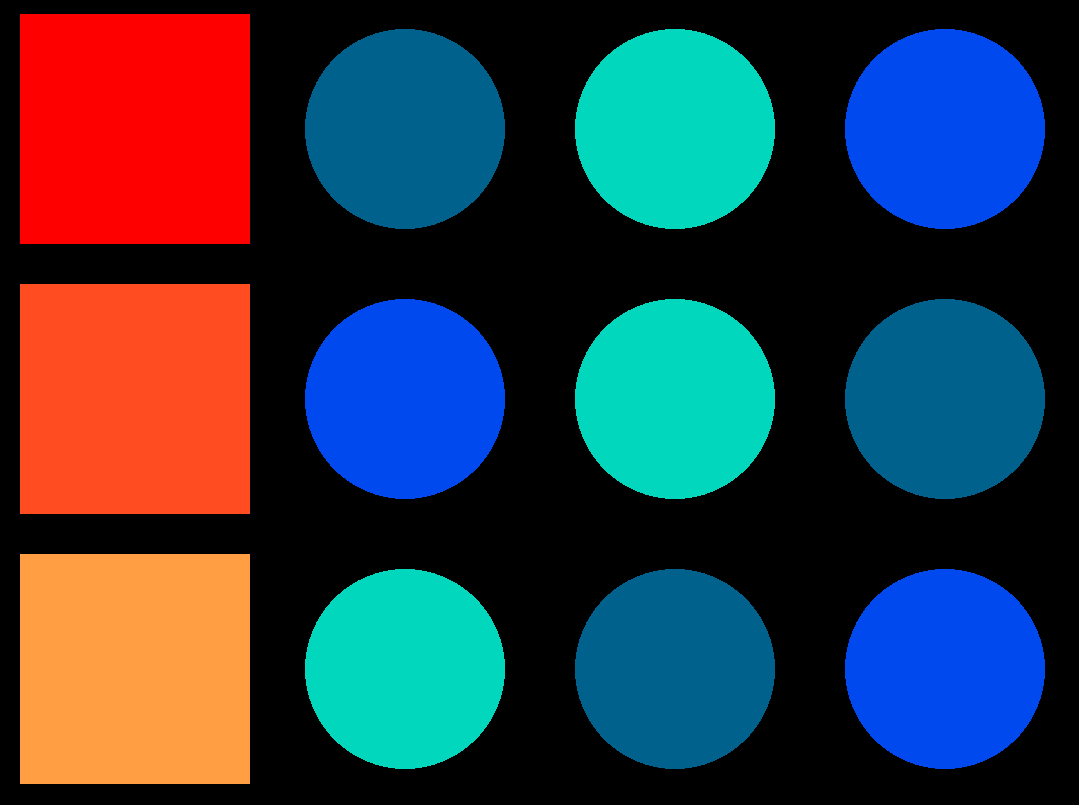
\includegraphics[width=0.3\linewidth]{prototype1}
\caption{Premier prototype d'interface de jeu}
\label{fig-prototype1}
\end{figure}

La sélection d'une préférence pour un des agents (l'allocation d'un objet à un agent) dessine un cercle de la couleur de l'agent derrière le cercle représentant la préférence en question. L'utilisateur peut donc choisir de sélectionner une certaine préférence en touchant le cercle correspondant. On note que le processus de sélection des ressources empêche de sélectionner plusieurs ressources pour un seul agent. À ce stade l'application est fonctionnelle.

Dans un soucis d'optimisation de l'espace et de lisibilité, la dernière modification structurelle de l'IHM consistait en la rotation de la grille de façon à ce que les agents se trouvent en haut et les préférences soient lues de haut en bas. Ce changement a permis l'utilisation d'une plus grande partie de la hauteur de l'écran et de pouvoir afficher de manière optimale les instances de plus grandes tailles (jusqu'à 7 agents) sur un grand nombre d'appareils.

L'étape suivante était de rendre l'interface agréable à l'œil et prête pour une distribution à plus grande échelle. Tous les changements décrit sont visibles en~\Cref{fig-finalgameview}. En premier lieu une harmonisation des couleurs a été opérée offrant une palette réduite pour favoriser la lisibilité du problème. Les données de l'instance en revanche ont pu revêtir une palette plus complète de couleurs et de formes pour que les joueurs puissent facilement distinguer entre les différents objets. Plusieurs symboles, variants en formes et en couleurs, ont été dessinés avec un faible niveau de détail pour ne pas fatiguer l'œil. Des barres verticales ont été ajouté pour chacun des agents ce qui facilite la distinction des préférences par agent et l'identifiant du niveau est montré en haut de l'écran. Nous avons voulu ainsi minimiser la quantité d'information à assimiler. Par exemple les agents ne montrent plus des couleurs différentes car ils sont déjà différenciés par leur position dans l'interface.

\begin{figure}[ht!]
    \centering
    \begin{subfigure}{0.34\textwidth}
        \centering
        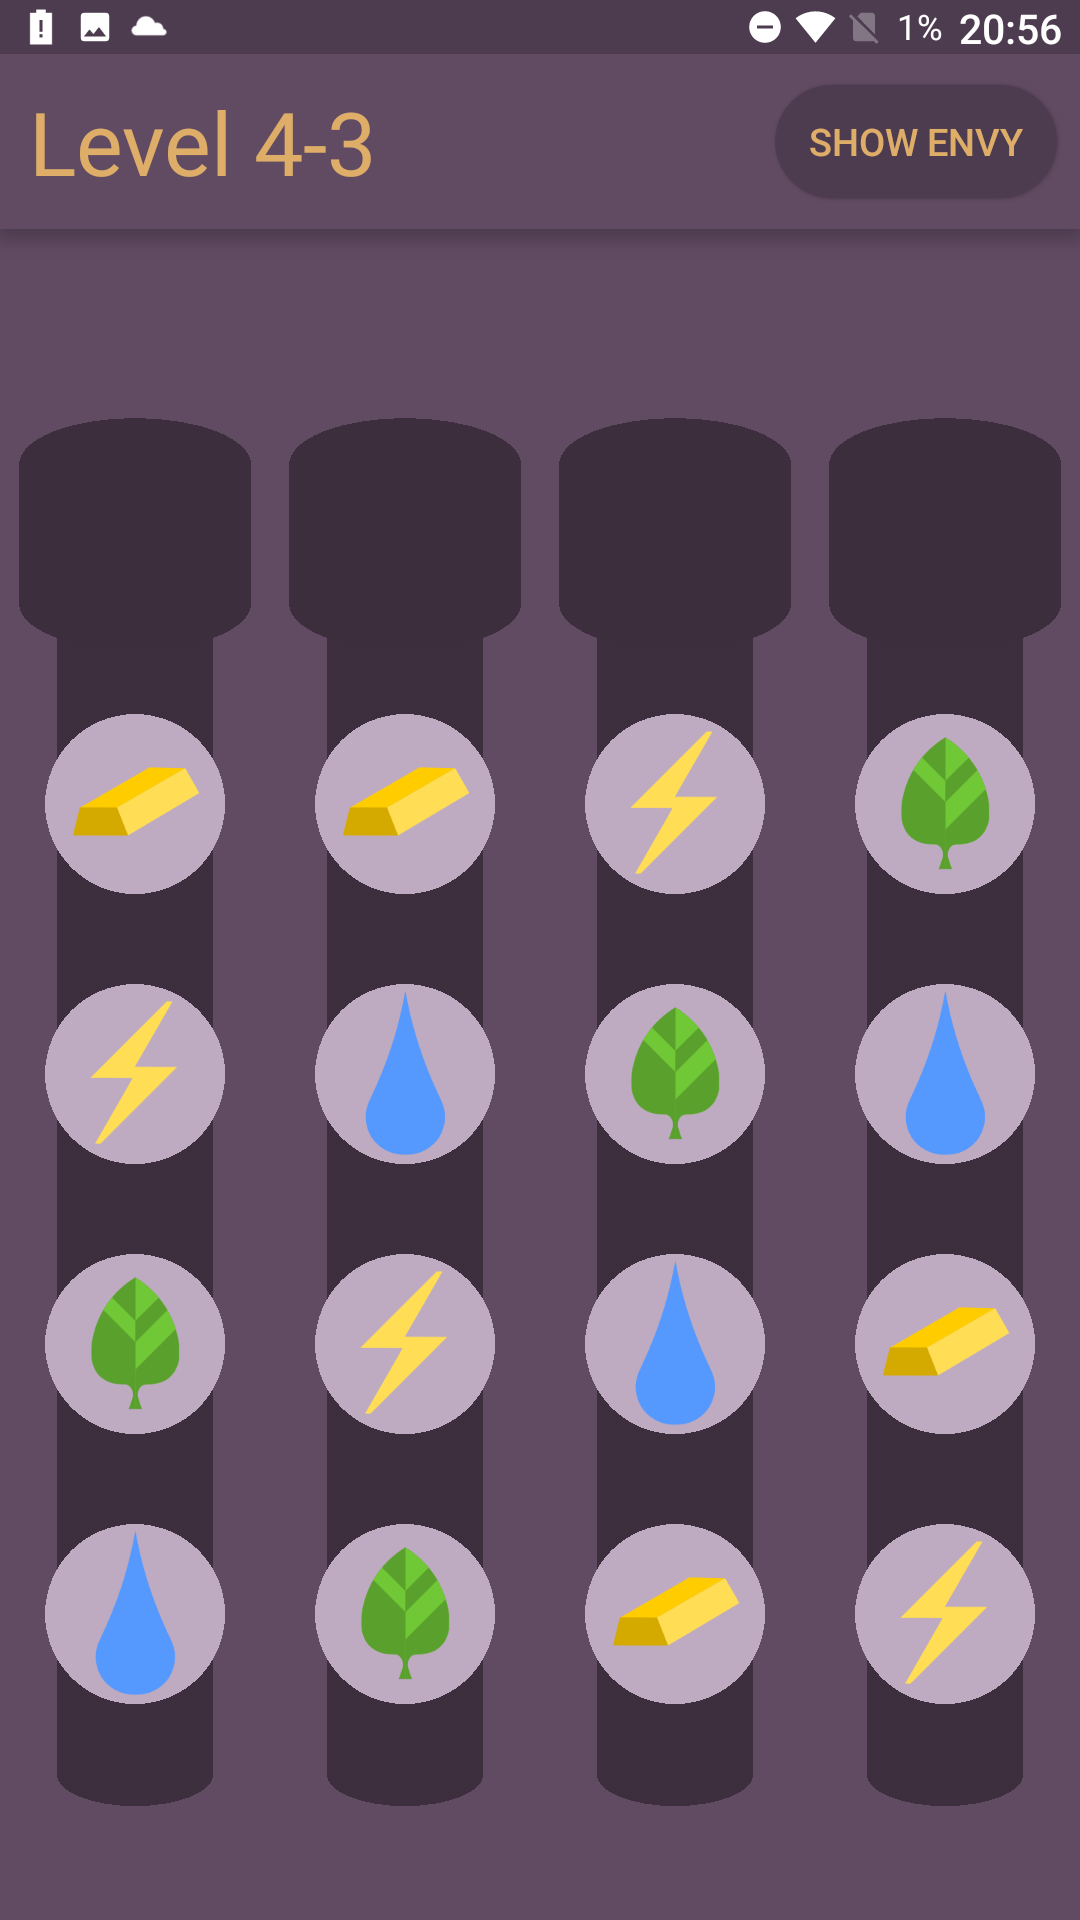
\includegraphics[width=\linewidth]{g1}
        \caption{Écran d'accueil}
        \label{fig-finalgameview}
    \end{subfigure}
    ~
    \begin{subfigure}{0.34\textwidth}
        \centering
        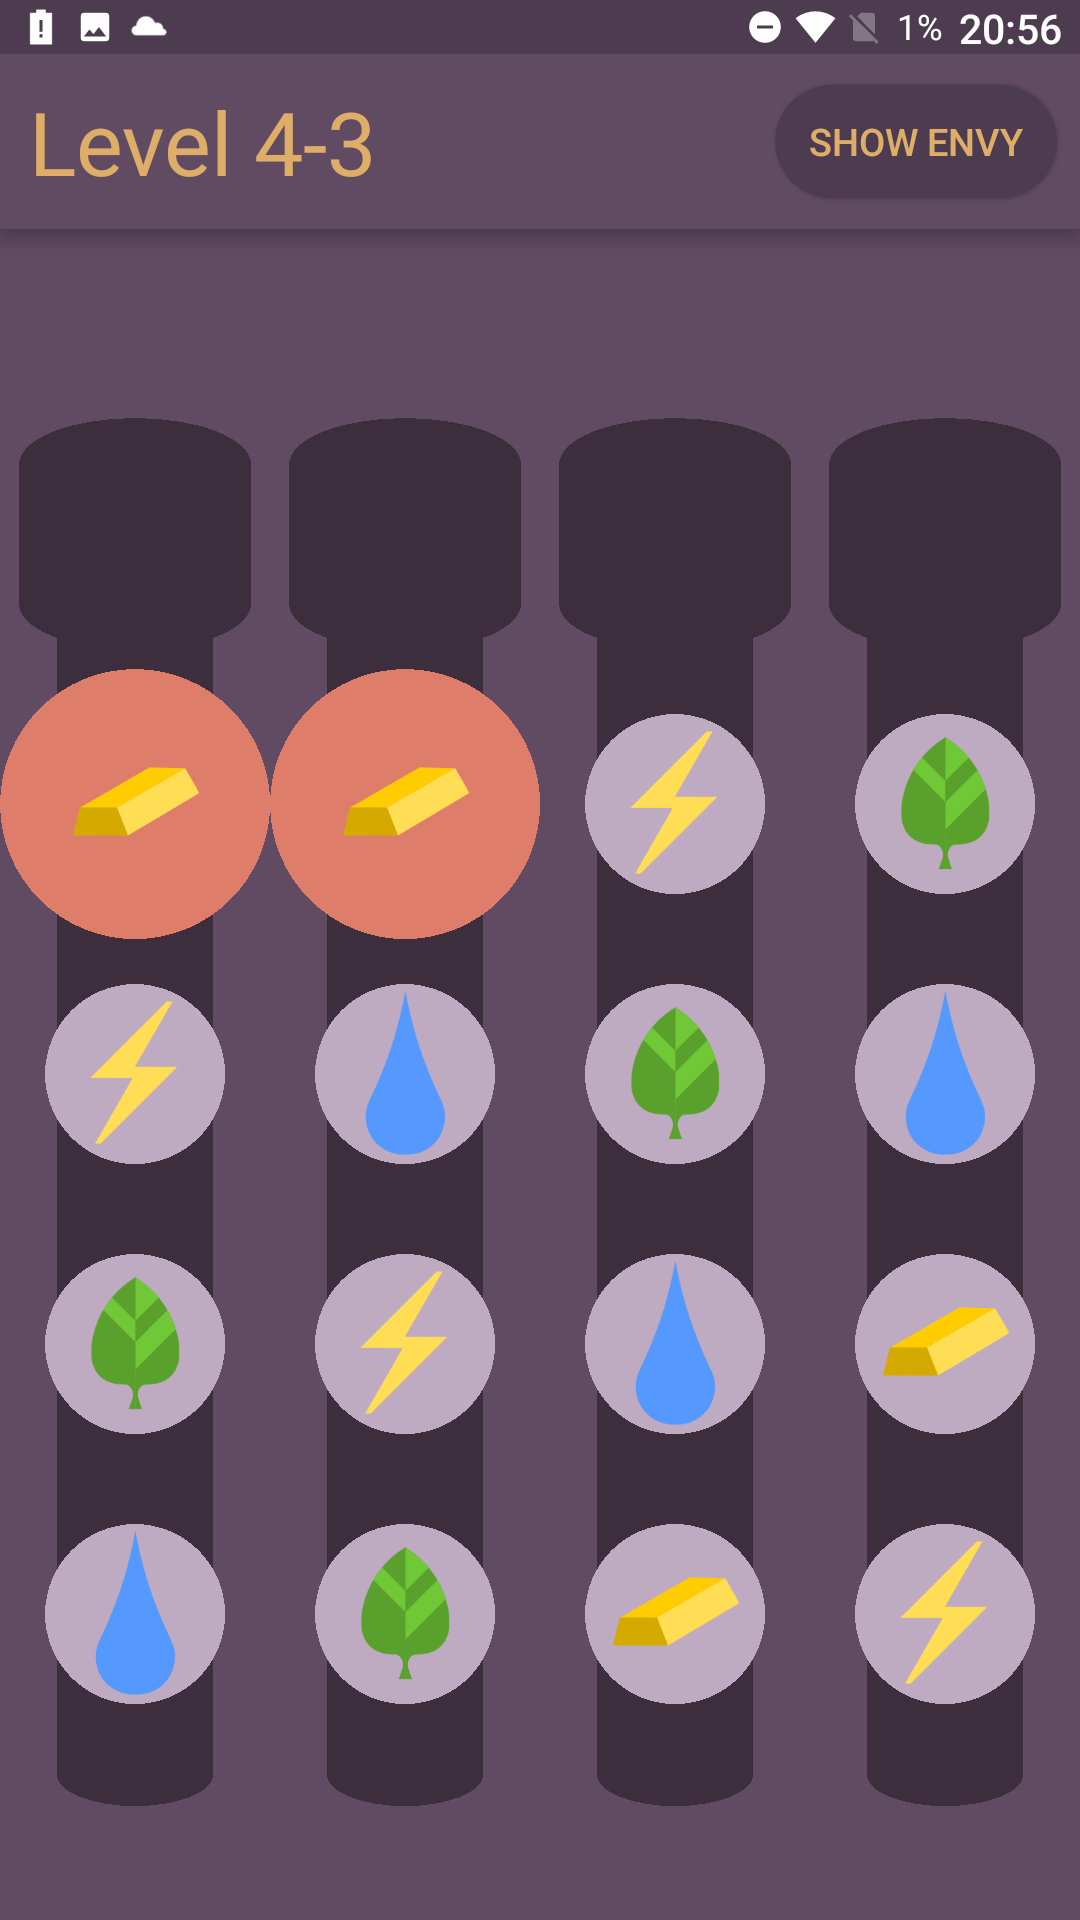
\includegraphics[width=\linewidth]{g2}
        \caption{Deux fois le même objet}
        \label{fig-twotimes}
   \end{subfigure}
    ~
    \begin{subfigure}{0.34\textwidth}
        \centering
        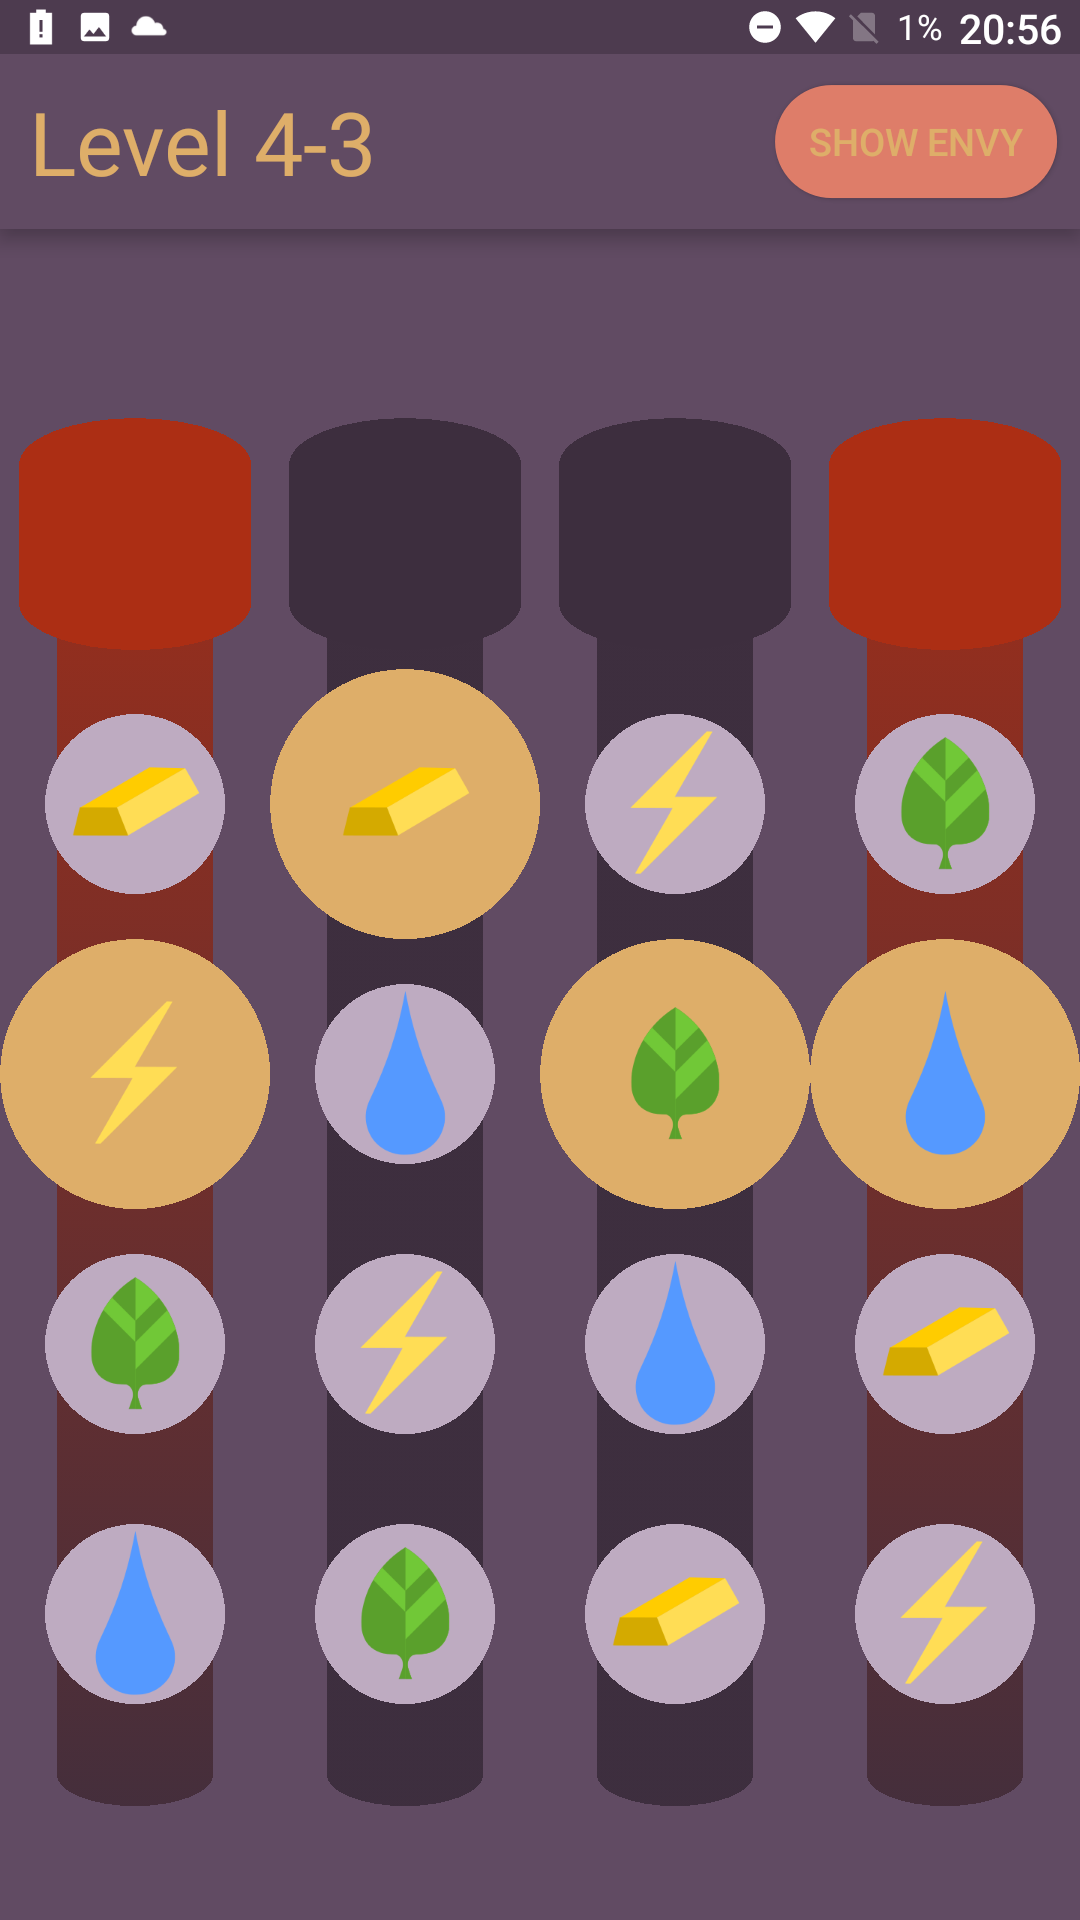
\includegraphics[width=\linewidth]{g3}
        \caption{Affichage de jalousie}
        \label{fig-envy}
    \end{subfigure}
    ~
    \begin{subfigure}{0.34\textwidth}
        \centering
        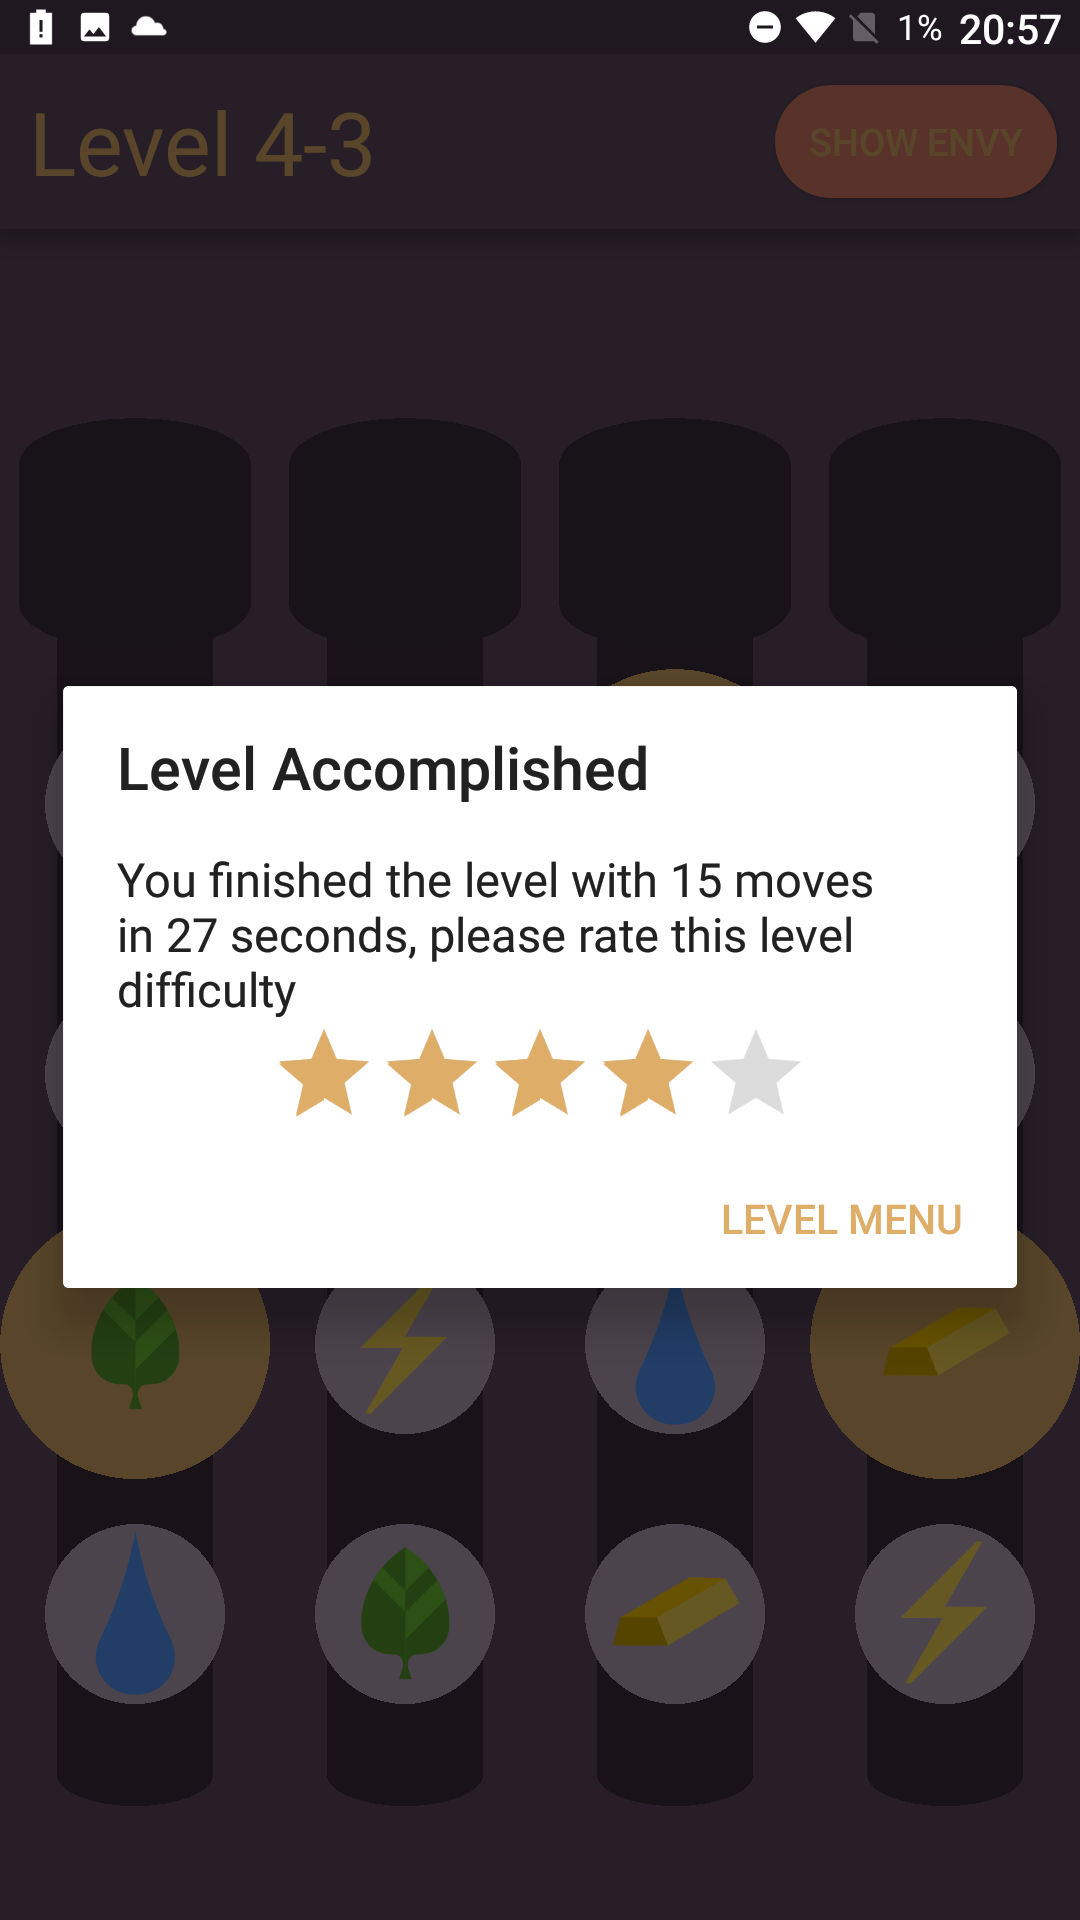
\includegraphics[width=\linewidth]{g4}
        \caption{Écran de victoire}
        \label{fig-victory}
    \end{subfigure}
    \caption{Interface de jeu finale}
\end{figure}

    Afin d'évaluer notre application, nous avons fait tester cette interface à nos proches. De multiples retours relataient ne pas comprendre quand et pourquoi une solution était erronée. Il était donc évident que pour améliorer l'expérience de jeu nous devions rendre la détection d'affectation non recevable plus aisée. Deux solutions ont été implémentées pour pallier ce problème. L'affichage d'une couleur différente lorsqu'une ressource est sélectionnée par deux agents ou plus permet au joueur de remarquer immédiatement qu'une telle assignation des ressources est impossible (\Cref{fig-twotimes}). La possibilité d'afficher en rouge les colonnes des agents jaloux améliore le potentiel d'amusement (\Cref{fig-envy}). Les joueurs passent moins de temps à rechercher pourquoi une solution n'est pas valide et plus de temps à chercher une meilleure solution. Notons que cette fonctionnalité facilite grandement le jeu, elle est donc désactivée par défaut et le joueur a la possibilité d'appuyer sur un bouton pour activer cet affichage.

    Ces deux additions rendent les résolutions plus aisées mais nous pensons que ces compromis permettent une expérience de jeu plus fluide, agréable et sans sentiment de confusion pour l'utilisateur, un point qui nous le rappelons, semble essentiel pour la distribution de l'application. Lorsqu'un niveau est résolu une fenêtre flottante annonce la victoire accompagnée du temps de résolution et du nombre de coups réalisés (\Cref{fig-victory}). Elle demande également à l'utilisateur de noter la difficulté ressentie pour le niveau en question. Ces données sont sauvegardées en ligne lorsque le joueur quitte la fenêtre.
    
    \subsubsection{Autres pages}
    
    Le reste de l'application devait comprendre un menu de sélection des niveau, une page profil, un tutoriel et une page \textquote{à propos} expliquant le projet. Ainsi dans la version finale de l'application, le \textbf{menu principal} (\Cref{fig-mainmenu}) est la première page sur laquelle arrive un utilisateur en ouvrant l'application. Il permet d'accéder à la liste des niveaux et aux autres pages citées ci-dessus. Le \textbf{menu de sélection des niveaux} (\Cref{fig-levelmenu}) catégorise les niveaux par nombre d'agents. L'utilisateur a la possibilité de jouer à tous les niveaux présentés et une pastille de texte indique si un niveau a été terminé ou commencé. La \textbf{page de profil} s'affiche au lancement de l'application lors de la première utilisation et est accessible depuis le menu principal. Elle permet, au moyen de deux zones de texte, de spécifier ou modifier les informations relatives au profil d'un joueur (âge, formation). Si un utilisateur ne souhaite pas divulguer ses informations il lui est possible de laisser les champs vides. Enfin la \textbf{page \textquote{à propos}} présente un bref résumé de l'objectif du projet et des raisons pour lesquelles l'application a été développée.
	
\begin{figure}[ht!]
    \centering
    \begin{subfigure}{0.3\textwidth}
        \centering
        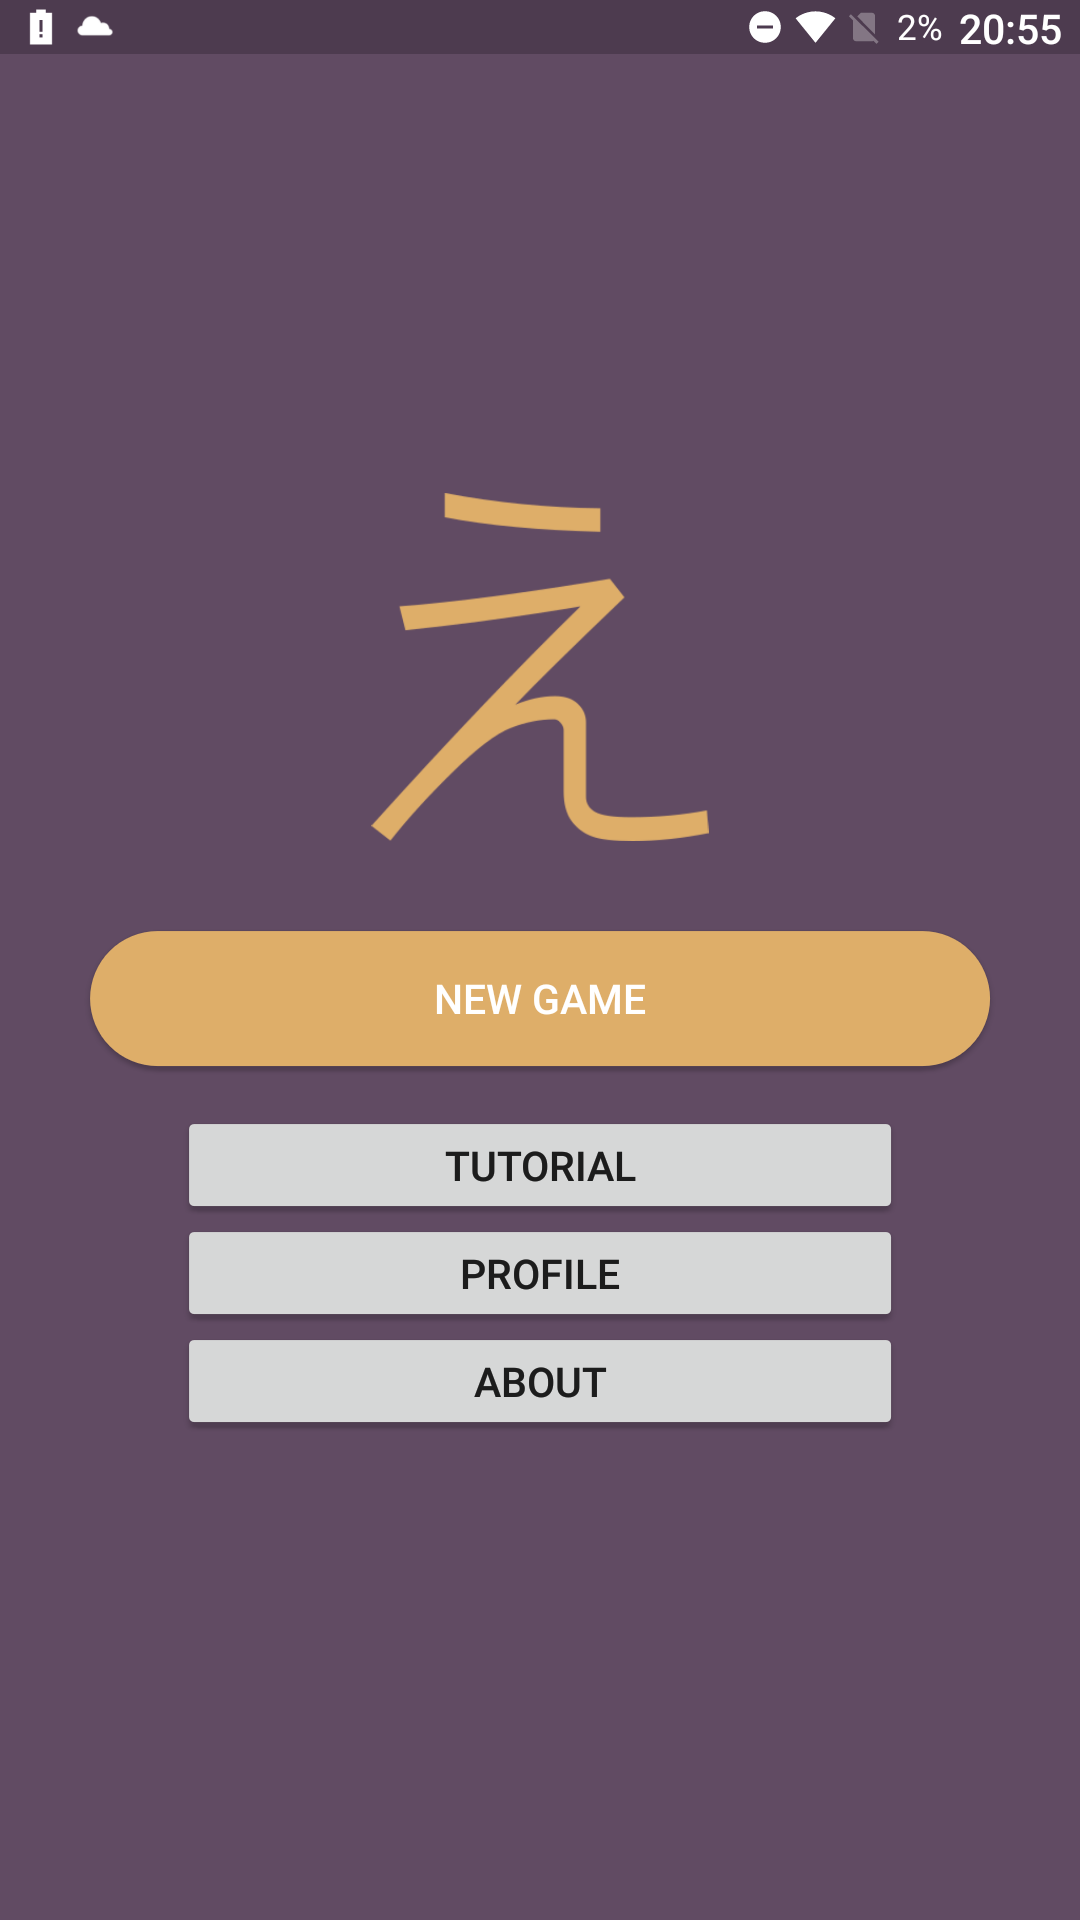
\includegraphics[width=\linewidth]{mainmenu}
        \caption{Menu principal}
        \label{fig-mainmenu}
    \end{subfigure}
    ~
    \begin{subfigure}{0.3\textwidth}
        \centering
        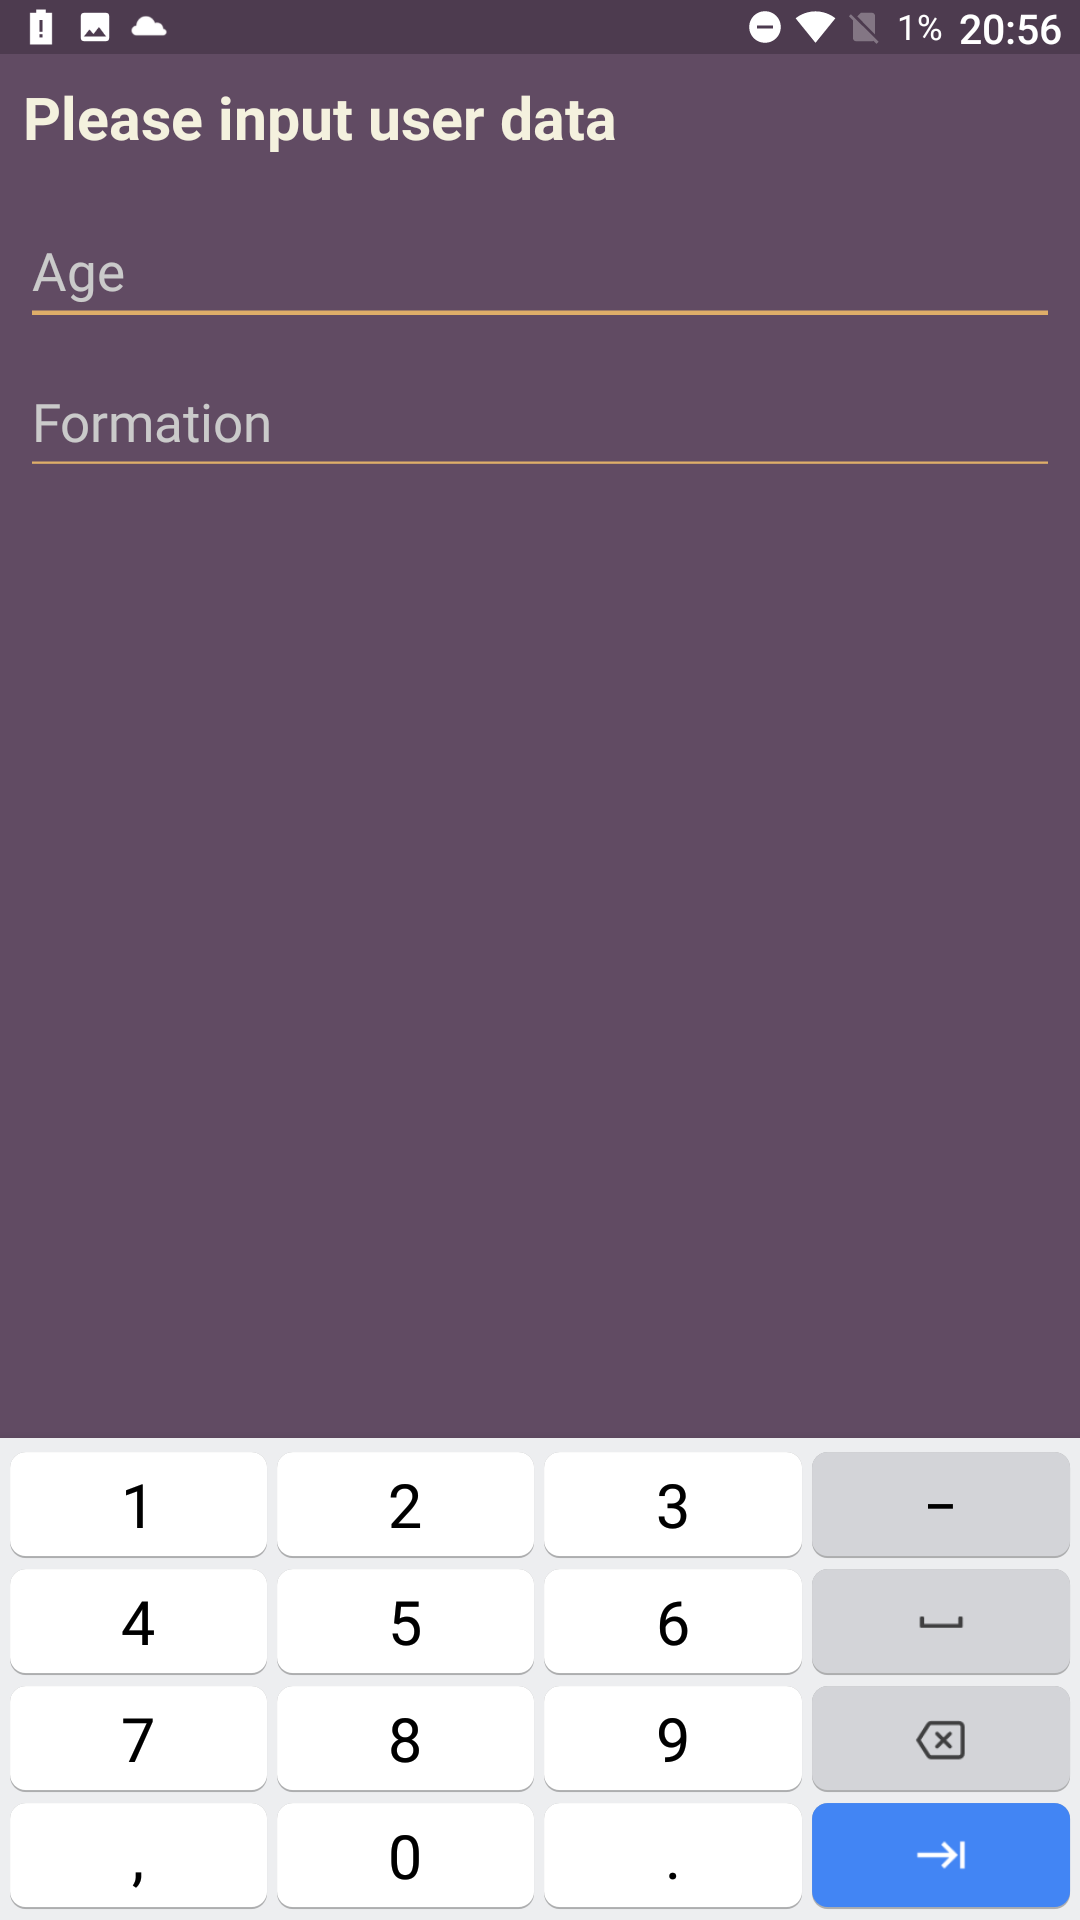
\includegraphics[width=\linewidth]{infor}
        \caption{Profil}
        \label{fig-profile}
    \end{subfigure}
    ~
    \begin{subfigure}{0.3\textwidth}
        \centering
        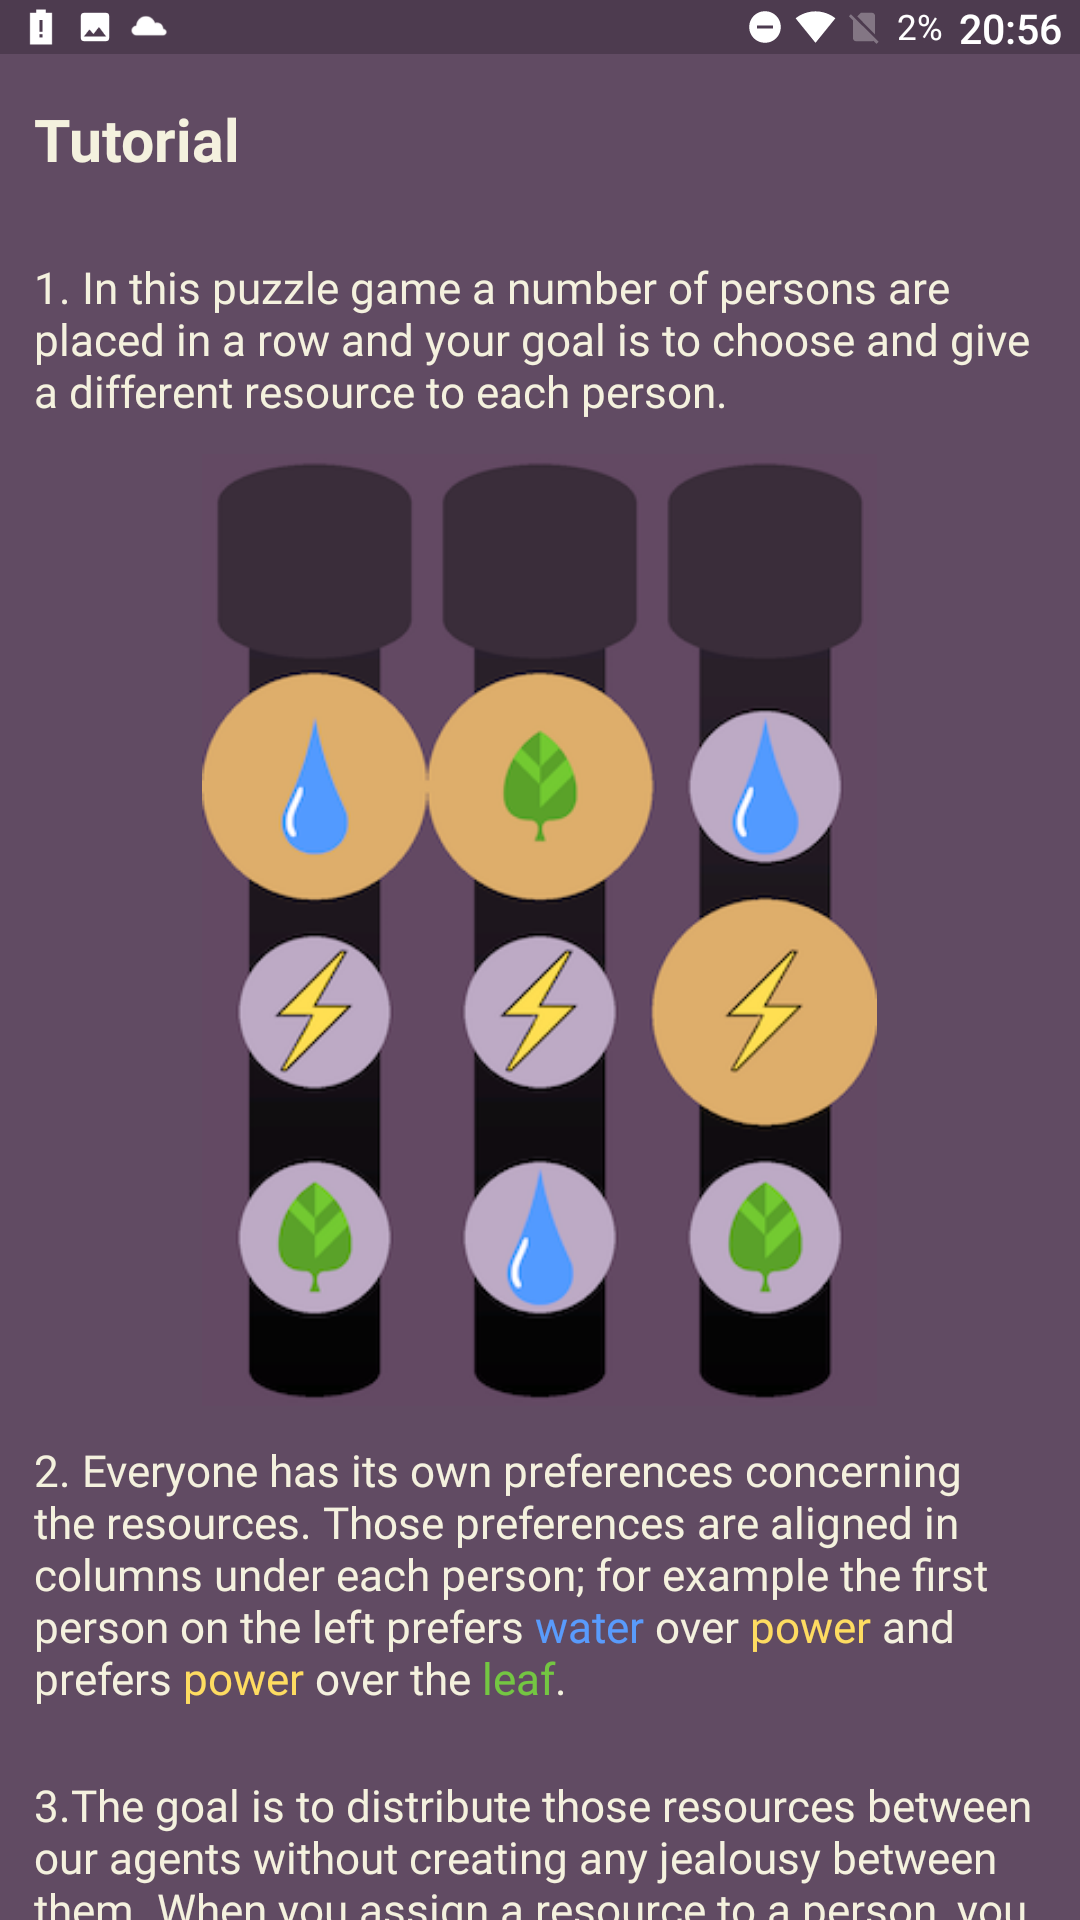
\includegraphics[width=\linewidth]{tuto}
        \caption{Tutoriel}
        \label{fig-tuto}
    \end{subfigure}
    ~
    \begin{subfigure}{0.34\textwidth}
        \centering
        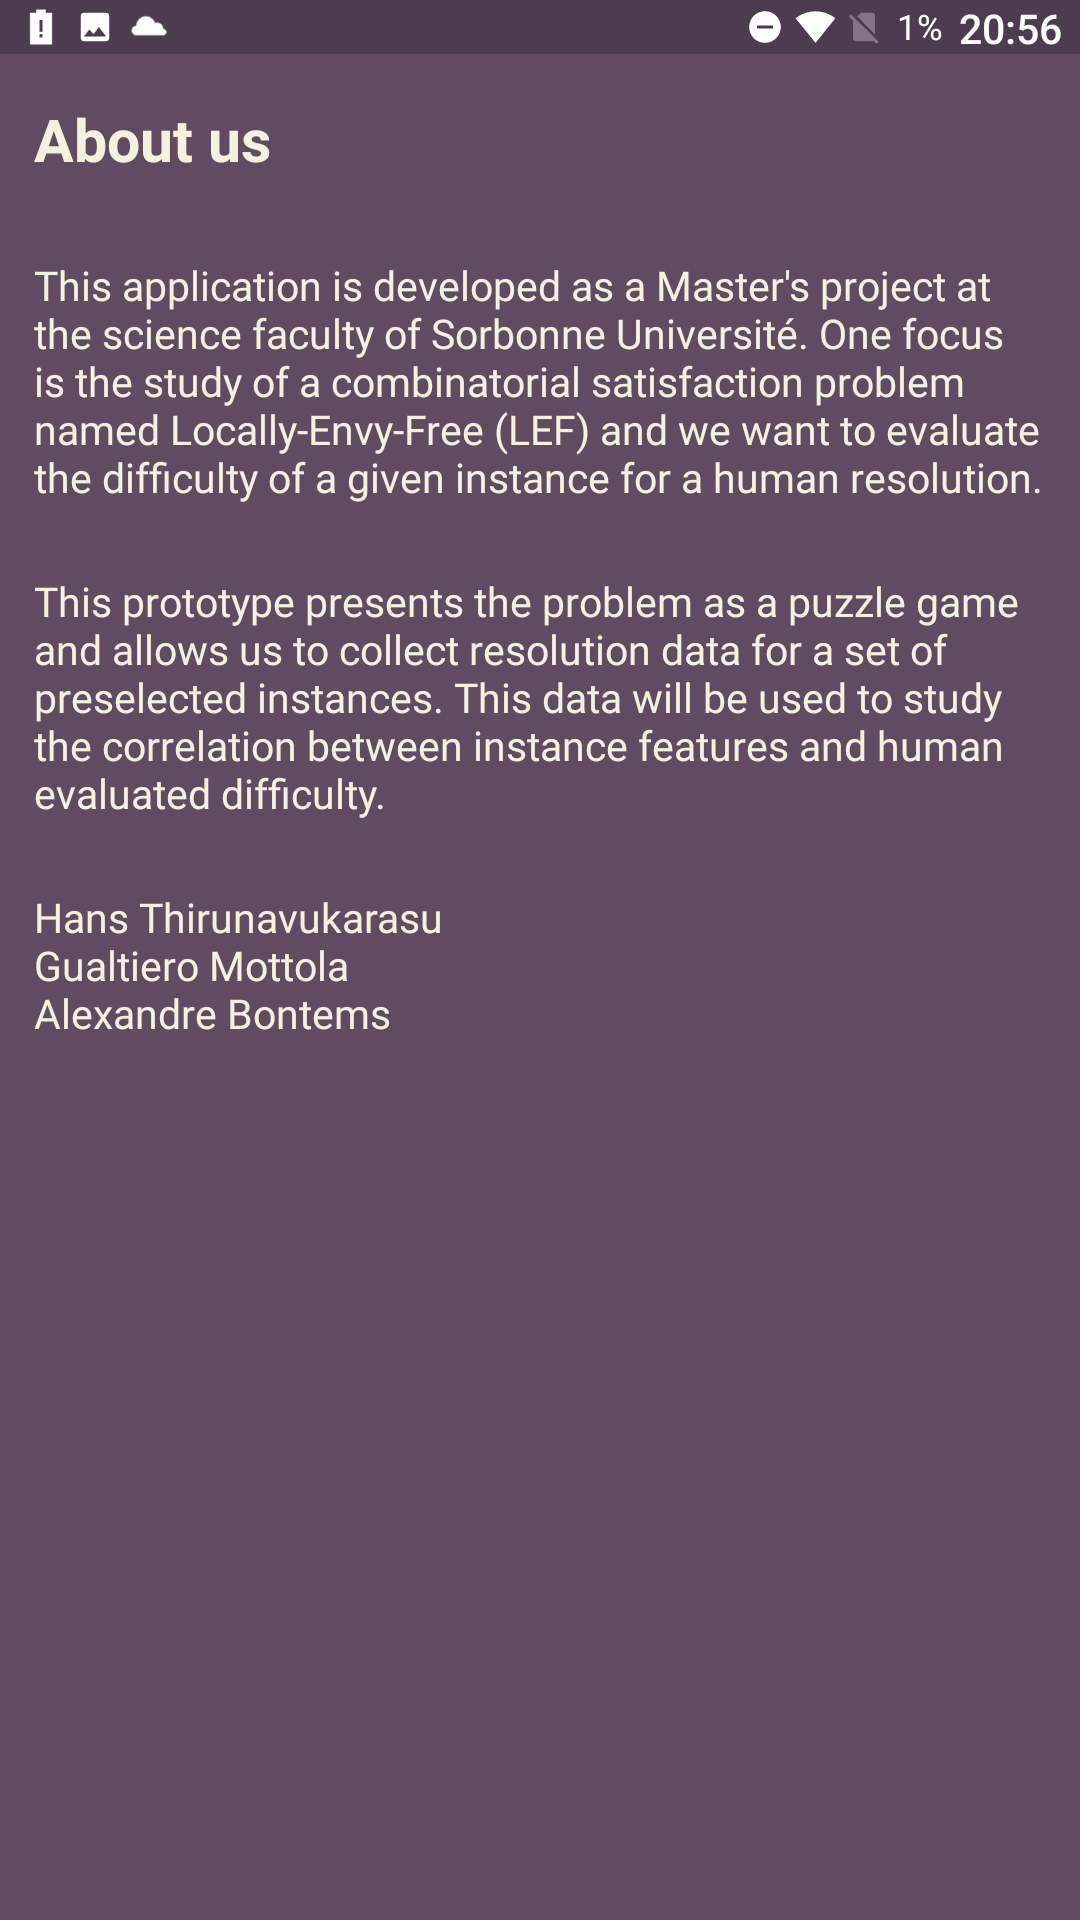
\includegraphics[width=\linewidth]{abou}
        \caption{About}
        \label{fig-about}
    \end{subfigure}
    ~
    \begin{subfigure}{0.34\textwidth}
        \centering
        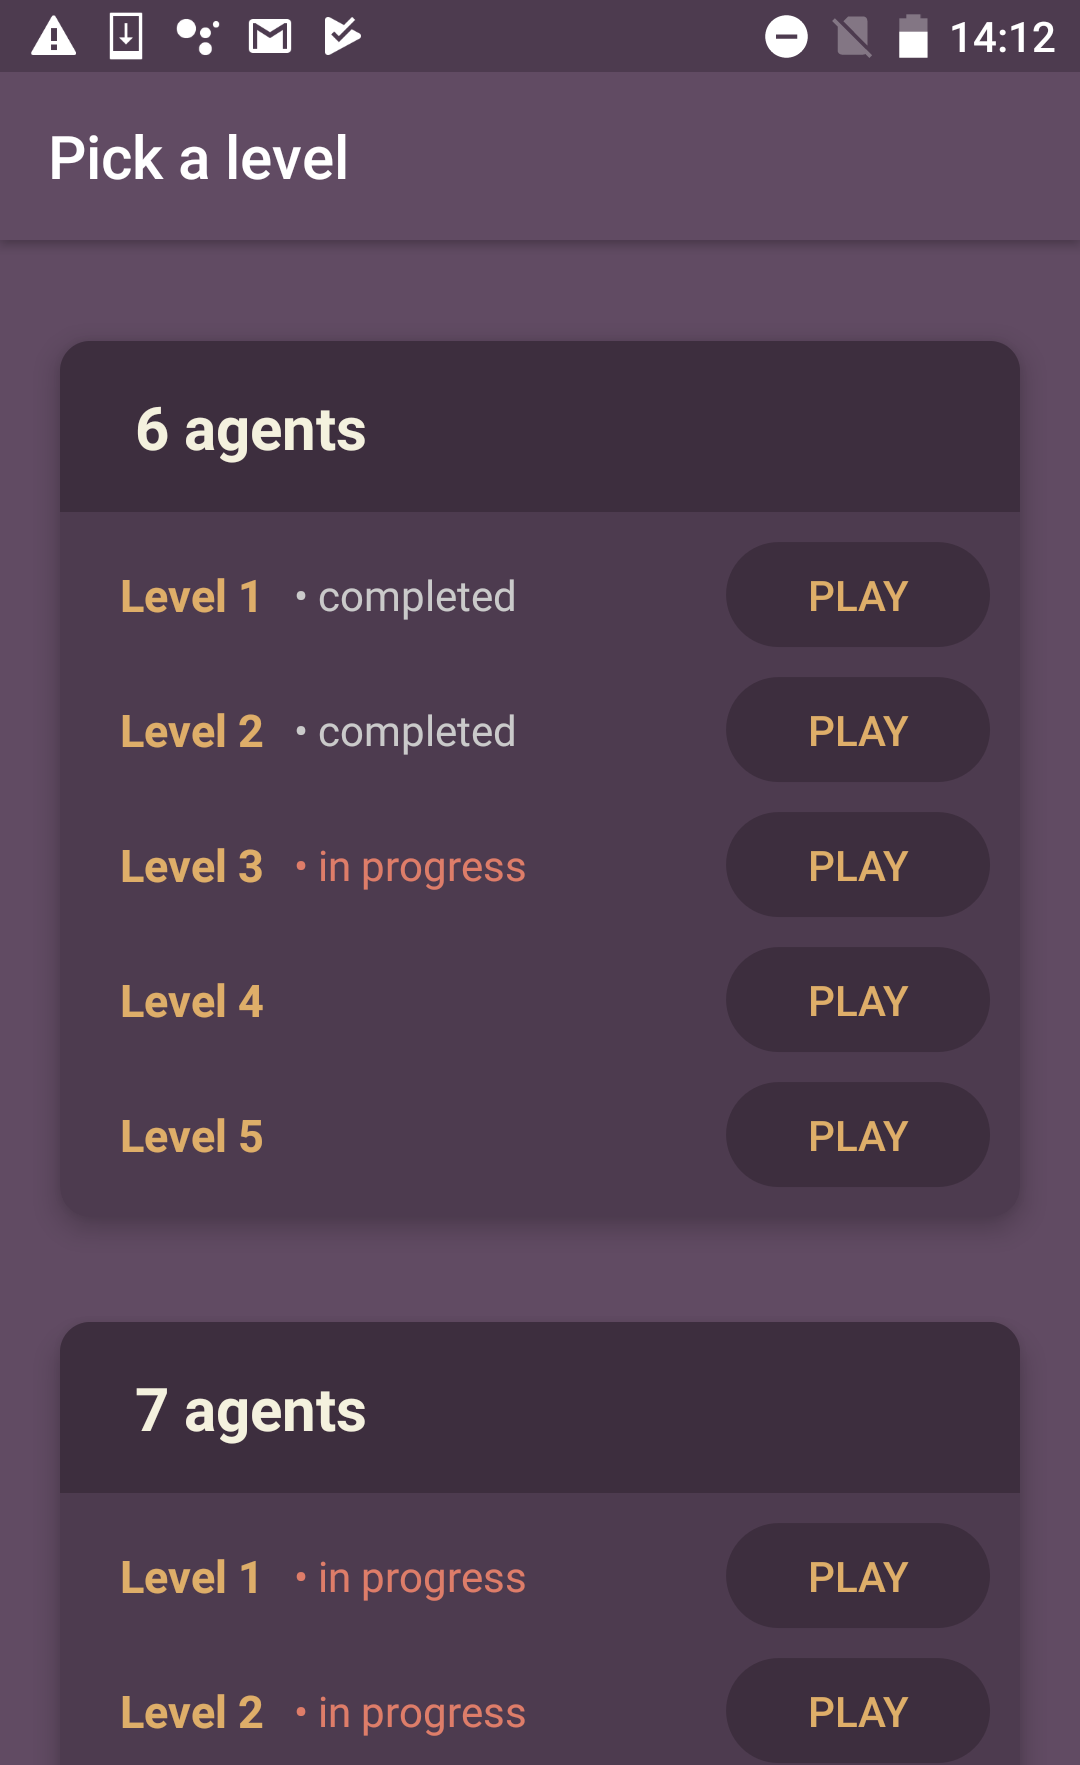
\includegraphics[width=\linewidth]{levelmenu}
        \caption{Sélection de niveau}
        \label{fig-levelmenu}
    \end{subfigure}
    \caption{Design final des menus de l'application}
    \label{fig-screen1}
\end{figure}

    \subsubsection{Tutoriel}
    
    Une composante très importante de l'application était le tutoriel permettant d'expliquer les règles du jeu. Une version interactive a d'abord été considéré qui aurait expliqué les actions nécessaires pour vérifier les contraintes tout en demandant à l'utilisateur de les effectuer. Par manque de temps cependant, une version combinant texte et images d'exemple a finalement été implémentée (\Cref{fig-tuto}). Il se déroule en trois étapes. Tout d'abord le but du jeu est explicité : trouver une allocation des objets pour les agents, un unique objet par agent. Ensuite les préférences sont abordées et les joueurs apprennent quel est l'ordre pour chaque agent. Enfin la notion de jalousie est montrée et expliquée à l'aide d'un exemple sous forme d'image. Le niveau servant d'exemple peut être retrouvé dans la liste des niveaux et peut être joué pour parfaire la compréhension. 
    
    Expliquer la notion d'envie à l'aide d'un court texte s'est révélé être un défi et plusieurs itérations se sont succédées avant que le tutoriel puisse être  considéré fonctionnel. Bien sûr il est probablement très améliorable.

	\subsection{Structure de l'application}
	\label{sec-struct}
	Une application Android s'organise en plusieurs composants et nous allons en présenter certains pour pouvoir décrire l'implémentation de l'application aisément. Nous allons notamment concentrer notre attention sur le concept d'activité, nécessaire à la présentation de l'interface.
	
	Une activité Android correspond à une fenêtre d'application et chaque application est donc composée d'au moins une activité. La navigation à l'intérieur d'une application se fait en changeant d'activité. Leur apparence visuelle est principalement définie par leur \textit{layout} qui structure l'agencement des vues (images, boutons, etc) et peut lier certains événements, initiés par l'utilisateur (comme par exemple un \textquote{clic} de bouton) à des actions prédéfinies (lancer un niveau par exemple). Le layout, chargé par une activité à sa création, est décrit dans un fichier XML.
	
Notre application est ainsi composée de six activités correspondant aux pages décrites plus haut: 
\begin{itemize}
    \item \texttt{MainMenuActivity},
    \item \texttt{LevelSelectActivity},
    \item \texttt{UserProfileActivity},
    \item \texttt{AboutActivity},
    \item \texttt{TutorialActivity},
    \item \texttt{GameActivity}.
\end{itemize}
Un bref Schéma de Navigation d'Interface (SNI) est disponible en~\Cref{fig-sni} (les conventions MACAO ne sont pas suivies).
\begin{figure}[ht!]
\begin{tikzpicture}
    \umlsimpleclass{MainMenuActivity}
    \umlsimpleclass[x=6]{LevelMenuActivity}
    \umlsimpleclass[x=12]{GameActivity}
    \umlsimpleclass[y=2]{TutorialActivity}
    \umlsimpleclass[y=-2]{UserProfileActivity}
    \umlsimpleclass[y=-2, x=6]{AboutActivity}
    
    \umlassoc{MainMenuActivity}{TutorialActivity}
    \umlassoc{MainMenuActivity}{UserProfileActivity}
    \umlassoc{MainMenuActivity}{LevelMenuActivity}
    \umlassoc{MainMenuActivity}{AboutActivity}
    \umlassoc{LevelMenuActivity}{GameActivity}
\end{tikzpicture}
\caption{SNI}
\label{fig-sni}
\end{figure}

	\subsection{Les modèles du jeu}

Nous allons ici décrire la partie back-end de l'application, en particulier les objets et classes utilisées pour représenter le jeu. Toutes les instances sont stockées dans un fichier XML et une classe \texttt{LevelLoader} permet de le \textit{parser} et charger les niveaux en mémoire vive. Le menu de sélection des niveaux qui est implémenté grâce à un \texttt{RecyclerView} peut alors être peuplé.

Le package \texttt{models} contient les classes nécessaires à la représentation du jeu dans l'application. On y trouve la classe \texttt{Level} construite à partir du XML et qui définit le nom d'un niveau, les préférences associées aux agents et sa taille. On y trouve aussi la classe \texttt{Model}, appelée dès lors qu'il est demandé de faire une modification du modèle (assignation d'un objet à un des agents par exemple). Cette classe est utilisée lorsqu'un joueur joue pour ne pas affecter la représentation en mémoire des niveaux. L'écran de jeu est rendu à partir d'un canevas pour faciliter l'ajout futur d'animations et autres éléments esthétiques. C'est pourquoi il a été nécessaire d'implémenter des classes pouvant être dessinées et représentant les différents éléments de la grille de jeu. Le package contient donc la définition de l'interface \texttt{IPiece}, implémentée par les classes \texttt{Preference} et \texttt{Actor} qui représentent respectivement les préférences et les agents.
\begin{itemize}
\item Définition d'une Pièce (interface \texttt{IPiece}) : cette interface est composé de deux méthodes; la méthode \texttt{getId} retourne l'identifiant de la pièce et la méthode \texttt{getPosition} permet de retourner la position de la pièce sous forme d'un objet position qui contient les indices de la ligne et de la colonne dans lesquelles se trouve la pièce.
\item Définition d'un Acteur (classe \texttt{Actor}) : cette classe implémente l'interface \texttt{IPiece} et toute ses méthodes. Elle représente les agents du jeu.                                                                                                                                                                                                                                                                                                                                      
\item Définition d'une Préférence (Classe \texttt{Préférence}) : cette classe implémente également l’interface \texttt{IPiece}. On y ajoute cependant là deux entiers: \texttt{value} (qui permet de déterminer de quel type est cette préférence) et \texttt{selectedby} (qui permet de savoir si cette préférence est sélectionnée par un des agents et par qui). 
\end{itemize}

Nous utilisions ensuite ces trois classes dans la classe \texttt{Model} décrite précédemment. Une des fonctionnalités que nous souhaitons mettre en valeur grâce à cette représentation est le calcul de la jalousie entre les agents. Il est très facile de récupérer des colonnes de la grille et de les comparer pour savoir si l'agent correspondant à cette ligne est jaloux. La fonction prends en arguments deux suites de préférences \textsf{P1} et \textsf{P2} et permet de détecter si l'agent \textsf{P2} est jaloux de l'agent \textsf{P1}. On commence par récupérer les préférences de chaque colonne et on vérifie qu'un objet a été alloué. Puis on compare la position de l'objet alloué à l'agent \textsf{P1} avec celle de \textsf{P2}; si l'objet de l'agent \textsf{P1} est préférée par l'agent \textsf{P2} a celui qui lui est assigné alors cette fonction retourne vrai. On note que cette méthode permet la détection de la victoire du jeu en calculant la jalousie de toute les paires d'agents côte à côte.

\begin{figure}[ht!]
\begin{lstlisting}
private boolean isJealous(Preference[] P1,Preference[] P2){
    if (P1[0] == null){
        return false;
    }
    Preference P2pref = null;
    Preference P1pref = null;
    for (Preference pref:P1){
        if(pref.getSelectedby() != -1){
            P1pref = pref;
        }
    }
    for(Preference pref:P2){
        if(pref.getSelectedby() != -1){
            P2pref = pref;
        }
    }
    if(P1pref == null || P2pref == null){
        return false;
    }
    for(Preference pref:P2){
        if(pref.getValue() == P1pref.getValue()){
            if(pref.getPos().getCol() < P2pref.getPos().getCol()){
                return true;
            }
        }
    }
    return false;
}
\end{lstlisting}
\caption{Fonction de détection de la jalousie}
\label{detection-jalousie}
\end{figure}

Une fonctionnalité de sauvegarde était nécessaire pour l'application. En effet lorsqu'un joueur commence un niveau sans finir de le résoudre il était d'une part important de conserver le temps passé sur ce niveau et pour rendre l'expérience plus agréable, de sauvegarder l'avancement dans la résolution. Un tel système a été implémenté à l'aide du système de \texttt{SharedPreferences} présent dans les applications Android. Il permet d'enregistrer des données persistantes et ainsi de garder en mémoire certaines informations même si l'application est quittée/fermée.

	\subsection{Récupération des données}
	
	Une fois l'application mobile réalisée, il nous fallait la faire tester sur un public de grande taille et offrant une certaine diversité pour recueillir des données pertinentes. Pour pouvoir réaliser l'apprentissage de difficulté décrit en~\Cref{sec-analyse}, il était demandé de pouvoir sauvegarder des données de résolutions sur une base de donnée distante. Le processus devait être automatique et silencieux de façon à simplifier au plus l'utilisation de l'application. Les serveurs Google et plus précisément le service GoogleSheets a été choisi pour cette tâche. 

Nous avons donc intégré dans l'application mobile, une solution permettant l'envoi de diverses données utilisateurs qui étaient enregistrées lors de la résolution d'une instance. L’API Google Sheets v4 permet l’écriture/lecture de données sur une feuille de calcul sur différentes plateformes : application mobile, site web, programme python, etc. La communication entre la feuille et notre application est géré et sécurisée via l’API. En effet elle utilise le protocole OAuth 2.0 pour autoriser les communications. Nous avons donc besoins d'identifiants, deux moyen sont disponibles :
\begin{itemize}
\item l’usage d’une Clé API,
\item l’usage d’un compte de service Google.
\end{itemize}

Néanmoins, la première méthode requiert une confirmation de l'utilisateur à chaque fois qu'il envoie des données via son téléphone. L'application demande alors la permission d'interagir avec la feuille sous le compte de l'utilisateur. Nous avons donc opté pour la seconde solution qui use d'un compte de service dédié à notre application. Celle-ci interagira via ce compte sans demander la confirmation de l'utilisateur, ce qui est crucial pour favoriser le côté \textquote{easy to use} de l'application. L'utilisateur est plus à même de vouloir tester notre application sur une courte durée/longue durée. Quelque soit la méthode, un fichier JSON contenant les identifiants est créé.\\

L'intégration de cette solution dans notre application se traduit donc par deux classes: \texttt{SheetsServiceUtil} et \texttt{GoogleSheetsWriteUtil}. La première contient une unique méthode \texttt{getSheetsService} qui permet la création de l’objet \texttt{Sheet}. C'est l'intermédiaire pour écrire et lire avec l'API. Cet objet contiendra les identifiants nécessaire à l'autorisation de la communication entre l'application et la feuille.

La deuxième classe \texttt{GoogleSheetsWriteUtil} contient toutes les méthodes qui seront appelées pour l'écriture de nos données. D'abord la méthode \texttt{setup} permet la création d'un objet \texttt{Credential} à partir de notre fichier JSON. Cette instance est ensuite utilisée dans la méthode \texttt{getSheetsService}.

Puisque les opérations réseaux sont asynchrones par nature, Android prohibe ce type d'action sur le thread principal de l'application. Ce thread est généralement dédiée à la mise à jour et affichage de l'interface. C'est pourquoi Android propose une classe \texttt{AsyncTask} utile pour effectuer des actions courtes sur un thread séparé. C'est la solution que nous utilisons pour envoyer nos données. Cela reste invisible à l'œil de l'utilisateur ce qui est à nouveau crucial pour le côté agréable et fluide de son expérience.

Nous avons donc trois classes dans \texttt{SheetsServiceUtil} qui héritent toutes de la classe \texttt{AsyncTask}:
\begin{itemize}
\item \texttt{WriteUserInfoAsyncTask},
\item \texttt{ModifyUserInfoAsyncTask},
\item \texttt{WriteUserEvalAsyncTask}.
\end{itemize}
Ces trois classes implémentent ainsi une méthode \texttt{doInBackground}, qui prend en paramètre une liste de chaîne de caractère, les données à envoyer, et qui réalise l'appel à l'API en tâche de fond. Nous appelons donc à l'intérieur les méthodes de l’API de Google Sheets pour mettre à jour (\texttt{ModifyUserInfoAsync}) ou écrire de nouvelles données (\texttt{WriteUserEvalAsyncTask} et \texttt{ModifyUserInfoAsyncTask}) dans notre feuille. Le code visible en~\Cref{fig-writeuser} montre un exemple d'utilisation de l'API.\\
\begin{figure}[ht!]
\begin{lstlisting}[tabsize=3]
private static class WriteUserInfoAsyncTask extends 
AsyncTask<String, Void, Void>{
	@Override
	protected Void doInBackground(String... data) {
		ValueRange body = new ValueRange()
                    .setValues(Arrays.<List<Object>>asList(
                            new List[]{Arrays.asList(data)}
                    ));
		try {
			AppendValuesResponse result = sheetsService.spreadsheets()
			.values().append(SPREADSHEET_ID, "User_Info!A1", body)
			.setValueInputOption("USER_ENTERED")
			.execute();
			Object userPos = result.getUpdates().get("updatedRange");
			prefs.edit().putString("userPos", (String) userPos).apply();
		} catch (IOException e) {
			Log.w("GoogleSheet", "Error during user info write; 
			rescheduling");
			failedUserInfo = data;
			e.printStackTrace();
		 }
		return null;
	}
}
\end{lstlisting}
\caption{Code permettant l'écriture des informations utilisateur}
\label{fig-writeuser}
\end{figure}

Comme il est possible que l’écriture des données sur la feuille puisse échouer (problème de réseau, téléphone non connecté à internet, etc), il est nécessaire de sauvegarder les données non envoyées pour permettre la planification d'un renvoi plus tard. Il existe donc pour cela deux variables listes dans la classe \texttt{SheetsServiceUtil}: \texttt{failedEvaluation} si l'écriture des données relative à une résolution échoue et \texttt{failedUserInfo} si l'écriture/modification du profil utilisateur échoue. 

Avant toute nouvelles écritures, il faut donc vérifier qu'il n'existe pas de données non envoyées. Pour cette raison, les trois méthodes gérant l'envoi de donnée font cette vérification. \texttt{writeUserInfo}, \texttt{modifyUserInfo} et \texttt{writerUserEval} appellent toutes, au début de leur exécution, une méthode \texttt{checkFailures} qui vérifie que les listes d'échecs soient bien vides. Si elles ne le sont pas, alors on crée de nouvelles \texttt{AsyncTask} pour renvoyer ces données avant de procéder à l'envoi des nouvelles données.

\begin{figure}[ht!]
\begin{lstlisting}[tabsize=3]
public void writeUserEvaluation(String... data) {
	this.checkFailures();
	new WriteUserEvaluationAsyncTask().execute(data);
}
\end{lstlisting}
\caption{Méthode writeUserEvaluation}
\label{fig-writeeval}
\end{figure}	
\end{document}